
%!TEX root = ../thesis.tex
%*******************************************************************************
%****************************** Third Chapter **********************************
%*******************************************************************************
\chapter{Reconstruction Framework of SBND}
\label{ChapterReco}

% **************************** Define Graphics Path **************************
\ifpdf
    \graphicspath{{Chapter6/Figs/Raster/}{Chapter6/Figs/PDF/}{Chapter6/Figs/}}
\else
    \graphicspath{{Chapter6/Figs/Vector/}{Chapter6/Figs/}}
\fi

%********************************** %Opening  **************************************

The process of extracting physics quantities from raw data recorded from an experiment is known as reconstruction.
At the Short-Baseline Near Detector (SBND), the physics characteristics of a particle can be reconstructed using multiple detection subsystems. 
For instance, a contained particle inside the Time Projection Chamber (TPC) might deposit energy resulting in only waveforms recorded by the TPC wire planes and the Photon Detection System (PDS).
On the other hand, an exiting particle might deposit additional energy in the Cosmic Ray Tagger (CRT) walls surrounding the TPC.
For a given particle, the TPC reconstruction extracts various quantities describing its topology, deposited energy and kinematics using charge information.
The PDS reconstruction provides additional high precision timing and deposited energy using light information.
The CRT reconstruction indicates if the particle is fully contained inside the detector.
As a result, reconstruction variables from all three detection subsystems are complementary to each other. 
%can be exploited for different analysis purposes such as cosmic rejection or particle identification.

This chapter provides a summary of the reconstruction framework at SBND.
Firstly, Section \ref{sec:reco_overview} gives an overview of the reconstruction workflow for each detection subsystem. 
The following Section \ref{sec:reco_tpc} details of the TPC reconstruction workflow, including a track-shower separation algorithm updated by the author.
The reconstruction of the PDS and CRT subsystem are summarised in Section \ref{sec:reco_others}.
Descriptions of some high level analysis tools using the reconstruction variables collectively from each detection subsystem are included in Section \ref{sec:reco_ana_tools}.                 
Finally, the chapter is concluded in Section \ref{sec:reco_concluding_remarks} with some remarks.

%********************************** %First Section  **************************************

\section{Overview of the Reconstruction Framework}
\label{sec:reco_overview}

%Describe the overall workflow
%Each detection subsystem in SBND requires a dedicated reconstruction workflow.
An overview of the reconstruction framework is illustrated in Fig. \ref{fig:Reco_Workflow}.
The TPC reconstruction workflow is shown by the red boxes.
This process begins with raw wire waveforms going through the signal processing performed by the Wirecell tool kit \cite{wirecell}.
This is followed by a hit finding algorithm to identify hits on the waveform.
Output hits are then used by the Pandora package \cite{pandora} to produce a 3D-reconstructed interaction, referred to as a \textit{slice}.
The PDS reconstruction workflow also follows a similar process to the TPC, as shown by the blue boxes.
A waveform deconvolution is first performed on raw PDS waveforms to filter noise.
Then, a hit finding algorithm identifies optical hits on the waveform and reconstruction is performed on the hits.
The equivalent output to the TPC-reconstructed interaction from the PDS reconstruction is referred to as a \textit{flash}.
Finally, the reconstruction for the CRTs is much simpler compared to the other two subsystems, consisting of only a hit finding and a reconstruction algorithm, as shown by the orange boxes.
The reconstruction variables from each detection subsystem are produced independently and can be matched together if they originate from the same interaction. 
The variables can also be combined and input into different high level analysis tools to extract more complex properties of the underlying interaction. 

\begin{figure}[htbp!] 
\centering    
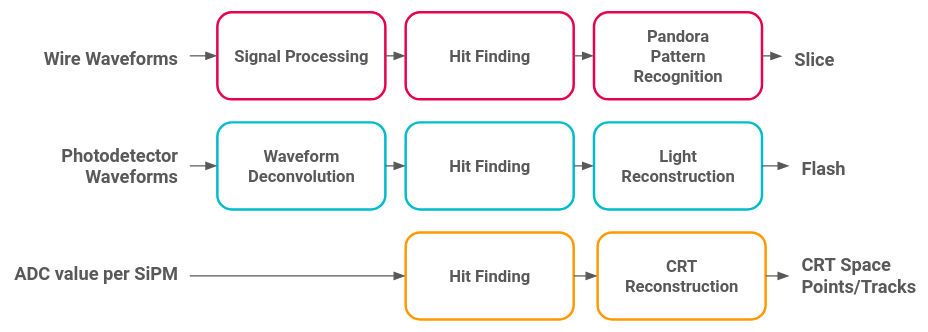
\includegraphics[width=1.0\textwidth]{Reco_Workflow}
\caption[Reconstruction Framework of SBND]{
Overview of the reconstruction workflow of the SBND detector.
}
\label{fig:Reco_Workflow}
\end{figure}

\section{Time Projection Chamber Reconstruction}
\label{sec:reco_tpc}

This section covers the TPC reconstruction workflow, starting with Section \ref{sec:signal_process} on the signal processing and hit finding.
Section \ref{sec:pandora} details the 3D reconstruction using Pandora and Section \ref{sec:trkshwbdt} delves into the track-shower separation algorithm  of Pandora. 

\subsection{Signal Processing and Hit Finding}
\label{sec:signal_process}

%Signal Processing
Signal processing is the first crucial step of TPC reconstruction, which is to deconvolve raw waveforms, accounting for detector effects such as noise, electronics response and field response. 
At SBND, signal processing is implemented using the WireCell tool kit \cite{wirecell}, which has been employed and developed by Liquid Argon Time Projection Chamber (LArTPC) experiments like MicroBooNE \cite{wirecell} and ProtoDUNE \cite{wirecell_protodune}.
%Both implementations here have demonstrated excellent performance to acquire deconvolved charge by performing deconvolution in time and wire dimension over the traditional deconvolution in time dimension only. 

The first step is noise filtering to remove excess and correlated noise from raw waveforms.
A 2D deconvolution of the field and electronics response is applied to recover the original charge deposited on the wire, where response functions consider the time response of a single wire as well as of neighbouring wires.
This step is particularly important for the induction planes to convert bipolar into unipolar signals, so that the integral of the waveform can be used for charge estimation.
High frequency filters are applied next to attenuate noise that is artificially amplified.
Finally, low frequency filters are utilised for peak finding and local baseline removal.

%Fig. \ref{fig:signal_processing_steps} shows an illustration of the signal processing steps.  
%In grey is the \textit{true} ionisation charge deposited on a wire, simulated without any detector effects applied.
%In red is the simulated raw waveform resulting from the deposited charge, convolved with noise, electronics and field response (See Section \ref{sec:wire_response}).
%The first step is noise filtering to remove the excess and correlated noise from raw waveforms.
%Then, the measured charge is deconvolved from the electronics and field response to recover the original charge deposited on the wire, as shown in orange.
%The deconvolution is 2D, where response functions consider the time response of a single wire as well as of neighbouring wires.
%This step is particularly important for the induction planes to convert bipolar into unipolar signals, such that the integral of the waveform can be used for charge estimation.
%
%High frequency filters are applied to attenuate noise that is artificially amplified, using Gaussian and/or Weiner filters depending on whether the signal is unipolar or bipolar.
%The example here is a bipolar waveform and therefore, has both filters applied, shown in yellow and green respectively.
%Then, low frequency filters are utilised for peak finding and local baseline removal, as shown in blue.
%Finally, the deconvolved waveform after baseline removal is shown in purple, which closely resembles the true charge as shown in grey.

\begin{figure}[b!]
\centering    
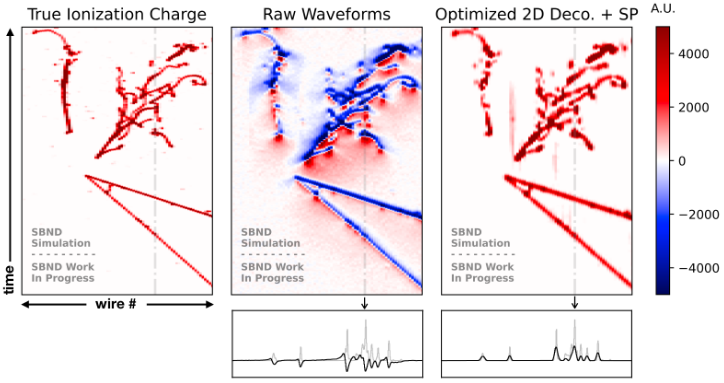
\includegraphics[width=0.85\textwidth]{signal_processing_waveform}
\caption[Event Displays of a Neutrino Interaction Before and After Signal Processing]{
Event displays of a simulated neutrino interaction using true charges (left), raw waveforms (middle) and deconvolved waveforms (right) \cite{LynnSignal}.
}
\label{fig:signal_processing_waveform}
\end{figure}
%This demonstrates the excellent performance of the signal processing chain to de-tangle detector effects from raw waveforms and recover the original deposited charge.  

Fig. \ref{fig:signal_processing_waveform} shows event displays of a simulated neutrino event as seen by wires on the induction plane.
The left panel depicts a neutrino interaction using the true charge deposition on wires, simulated without any detector effects applied.
The middle panel illustrates the interaction using raw waveforms before signal processing.
The right panel shows the interaction using deconvolved waveforms after signal processing.
Two tracks and two showers can be clearly seen in the right panel, demonstrating the excellent performance of the signal processing chain to de-tangle detector effects from raw waveforms and recover the original deposited charge.
Signal processing in SBND is currently a work in progress, as labelled so in Fig. \ref{fig:signal_processing_waveform}.
At the time of writing, optimisation signal processing specifically for the SBND electronics has begun.

%\begin{figure}[ht!] 
%\centering    
%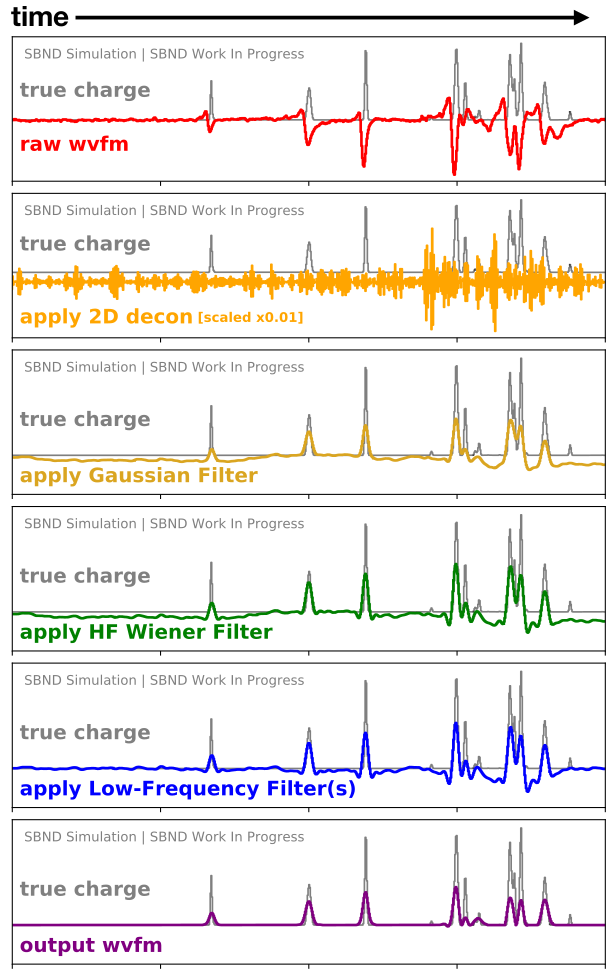
\includegraphics[width=0.45\textwidth]{signal_processing_steps}
%\caption[Signal Processing Steps]{
%Steps of signal processing applied to a bipolar raw waveform \cite{LynnSignal}.
%}
%\label{fig:signal_processing_steps}
%\end{figure}
%\vspace{0.5cm}

%\subsection{Hit Finding}
%\label{sec:hit_find}

Hit finding is to search for Gaussian-shaped pulses above a threshold, by fitting a series of Gaussians to the deconvolved waveform  \cite{gaushitfinder}.         
The number of pulses is determined by the number of maxima found when differentiating the waveform, where each pulse represents a hit. 
Fig. \ref{fig:gaushit} demonstrates the hit finding process for a deconvolved waveform, showing four identified hits and each fitted with a Gaussian.
Information of the fit is extracted and used by downstream reconstruction.
The peak time represents the time at which the charge arrives at the wire, used for determining the drift position and matching hit coincidence across wire planes.
The height and the width of the Gaussian are used to calculate the integral of the pulse, representing the deposited charge on the wire, subsequently used in downstream analysis for energy deposition computation.

\begin{figure}[htbp!] 
\centering    
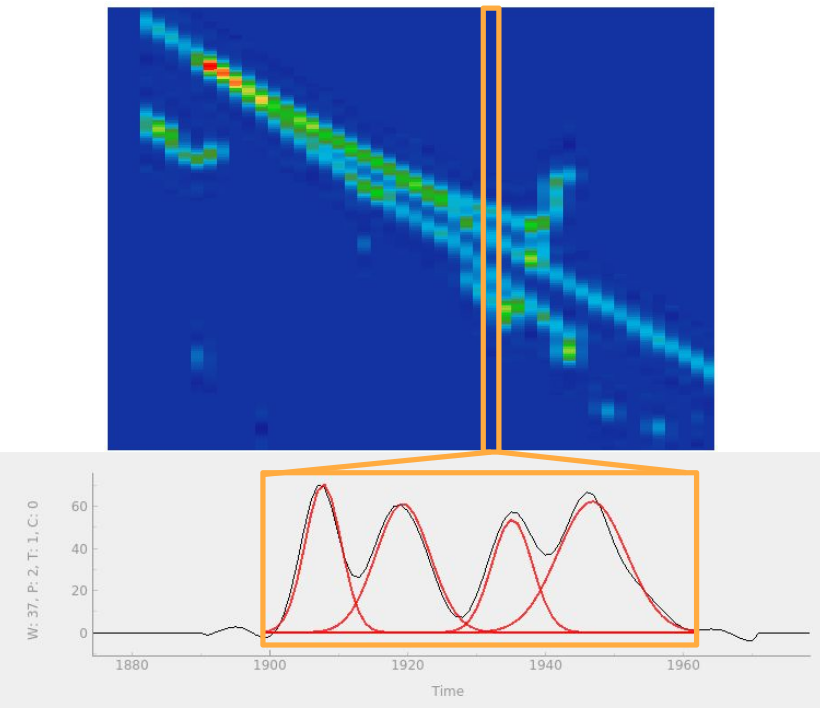
\includegraphics[width=0.45\textwidth]{gaushit}
\caption[Hit Finding Diagram]{
Diagram illustrating the hit finding algorithm on a single wire \cite{EdPhD}.
}
\label{fig:gaushit}
\end{figure}

\subsection{Pandora Pattern Recognition}
\label{sec:pandora}

%Pattern Recognition: Pandora
Output hits are used for 3D reconstruction, performed by the Pandora pattern recognition package \cite{pandora}.
It was first developed for the International Linear Collider and later extended to LArTPC experiments.
The package is made up of over 100 individual algorithms, each performing a specific task along the reconstruction chain.
Output from Pandora represents an interaction, referred to as a \textit{slice}, containing a hierarchy of particles starting with a neutrino parent at the interaction vertex.

The reconstruction begins with a workflow to reconstruct cosmic-like objects that leave long tracks inside the detector.
Hits on each wire plane independently are grouped together to form 2D clusters.
Clusters across planes are matched to perform 3D reconstruction under the assumption that all clusters are track-like.
A cosmic rejection is performed to identify if a cluster is cosmic-like or neutrino-like, although it is deliberately cautious at this stage so that only very unambiguous cosmic-like clusters in nature are removed.

The remaining clusters are input into a second workflow dedicated towards neutrino reconstruction.
It begins with a slicing algorithm that group clusters into \textit{slices}, where each slice encapsulates hits coming from a single origin, representing an interaction.
2D clustering is re-performed on each wire plane independently, with a new assumption that clusters can be both track-like and shower-like.
A vertexing algorithm identifies the interaction vertex of the slice and its associated clusters.
A series of pattern matching algorithms grows the interaction starting from the vertex and performs 3D reconstruction by matching 2D clusters across different planes.
Output 3D reconstructed objects in a slice associated with a vertex represent \textit{particles}.

At this stage, a \textit{track score} is assigned to a particle if it has a track-like or a shower-like topology, which is determined by a Boosted Decision Tree (BDT).
Development of the track-shower separation BDT is covered in Section \ref{sec:trkshwbdt} next.
Both track and shower reconstruction algorithms are performed on the particle. 
Finally, a hierarchy algorithm classifies the hierarchy of particles in a slice, starting with the neutrino parent vertex, and other particles are children, grandchildren, etc. of the parent.

%Calorimetry reconstruction
The last stage is energy deposition computation of the reconstructed particles.
Both track and shower energy computations first convert ADC units to charges by multiplying by a charge calibration constant.
The track energy is computed from charge using the modified Box recombination formalism, factoring in the electric field distortion (See Eq. \ref{eq:recomb_modbox}, Section \ref{sec:simDeltaRay}).
The shower energy is computed from charge by multiplying by a shower calibration constant, factoring in an averaged recombination factor regardless of the electric field.
Once SBND is operational, the charge calibration constant is expected to be measured using anode-to-cathode crossing cosmic muons while the shower calibration constant can be acquired from the neutral pion invariant mass as a standard candle \cite{uboone_gamma}.

\subsection{Track-Shower Separation Boosted Decision Tree}
\label{sec:trkshwbdt}

Reconstructed particles from Pandora are assigned a track score determined by a BDT, configured as a binary classification tool.
The track score spans between 0 and 1 such that if a particle has a very high track score close to 1, it is track-like.
Otherwise, if its track score is very close to 0, it is shower-like.

The track-shower BDT became more important in the reconstruction as well as the analysis due to a new paradigm introduced by Pandora, where both track and shower reconstruction are performed on a particle regardless of its track score.
All reconstructed particles now have two sets of reconstruction variables for track-like and shower-like.
Users have the freedom to decide which variables to use depending on their signal topology, and thus not pre-determined by Pandora.
The track score can inform which appropriate reconstruction variables should be used for the analysis. 

The original track-shower separation BDT included variables describing the topology of a particle such as its length, distance and direction with respect to the parent vertex, as well as calorimetry variables describing the charge distribution of the particle.
More details of the input variables and the training of the BDT can be found in Ref. \cite{EdPhD}.
It was updated to extend to a brand new set of variables describing how cone-like the charge distribution of a particle is as well as a new variable describing the particle hierarchy.

The cone variables were first developed in Ref. \cite{warwick_pid} for particle identification and were imported into Pandora for reconstruction purposes.
There are three variables: (1) halo-total ratio, (2) concentration and (3) conicalness as depicted in Fig. \ref{fig:cone_variables}.
The diagrams depict the hit distribution of a particle, where each circle represents a hit associated with a charge value and the star represents the vertex of the hit cluster.
The illustration is in 2D for simplicity, however the variables are computed in 3D.

The first variable is the halo-total ratio, illustrated in Fig. \ref{fig:halototalratio}.
The Moliere radius in liquid argon is 10 cm, defined such that average 90\% of a cylindrical energy deposition is contained within this radius \cite{Passage}.
The region outside the Moliere radius is considered the halo region.
The hits in the halo are shown as green circles whereas any other hits are shown as grey circles.
The halo-total ratio is then defined as:
\begin{equation}
	\mathrm{Halo\ - Total\ Ratio = \frac{Charges\ in\ the\ Halo}{Total\ Charges}}.
\end{equation}

The second variable is called concentration, accounting for how concentrated the charge distribution is to the centre of the cluster.
This is depicted in Fig. \ref{fig:concentration}, where each hit is assigned a colour showing how weighted it is with respect to its orthogonal distance to the cluster direction.
The closer the hit to the centre, the more weighted it is.
The concentration variable is defined as the total weighted charges divided by the total charge as following:
\begin{equation}
	\mathrm{Concentration = \frac{\sum Charge \times Weight}{Total\ Charges}}.
\end{equation}

Finally, the conicalness variable examines the hit distribution at the end and the start of the cluster as depicted in Fig. \ref{fig:conicalness}. 
It is defined as the ratio between the concentration at the end of the cluster compared to that at the start of the cluster:
\begin{equation}
	\mathrm{Conincalness = \frac{Concentration\ at\ the\ End}{Concentration\ at\ the\ Start}}.
\end{equation}

\begin{figure}[hb!]
        \centering
        \begin{subfigure}[b]{0.495\textwidth}
            \centering
            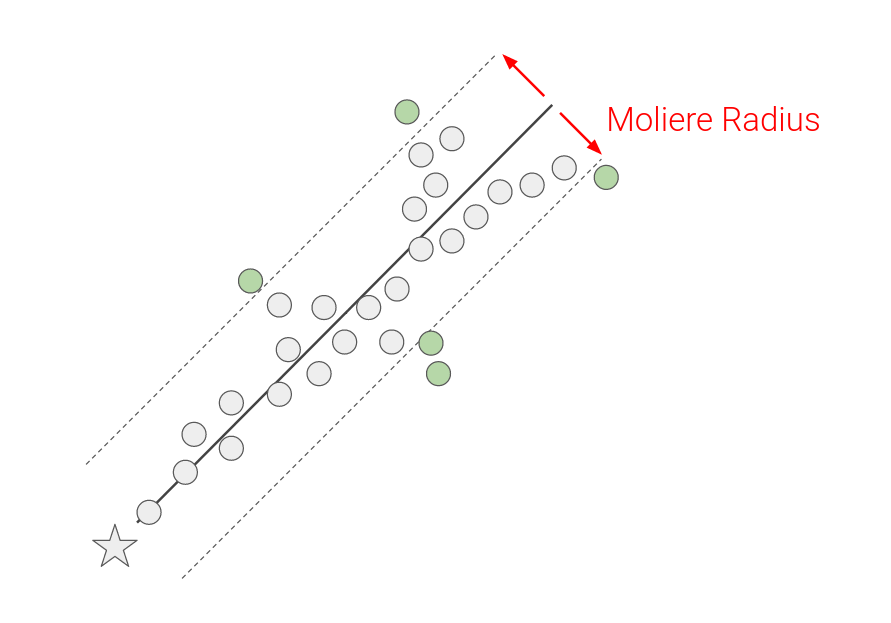
\includegraphics[width=\textwidth]{HaloTotalRatio}
            \caption{Halo-Total Ratio}%
            \label{fig:halototalratio}
        \end{subfigure}
        \hfill
        \begin{subfigure}[b]{0.495\textwidth}  
            \centering 
            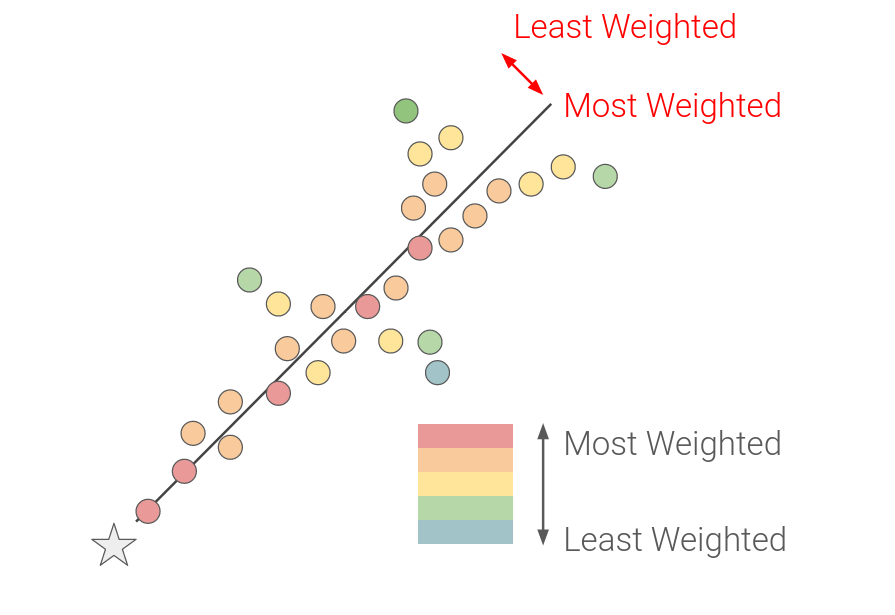
\includegraphics[width=\textwidth]{Concentration}
            \caption{Concentration}%
            \label{fig:concentration}
        \end{subfigure}
        \hfill
        \begin{subfigure}[b]{0.495\textwidth}  
            \centering 
            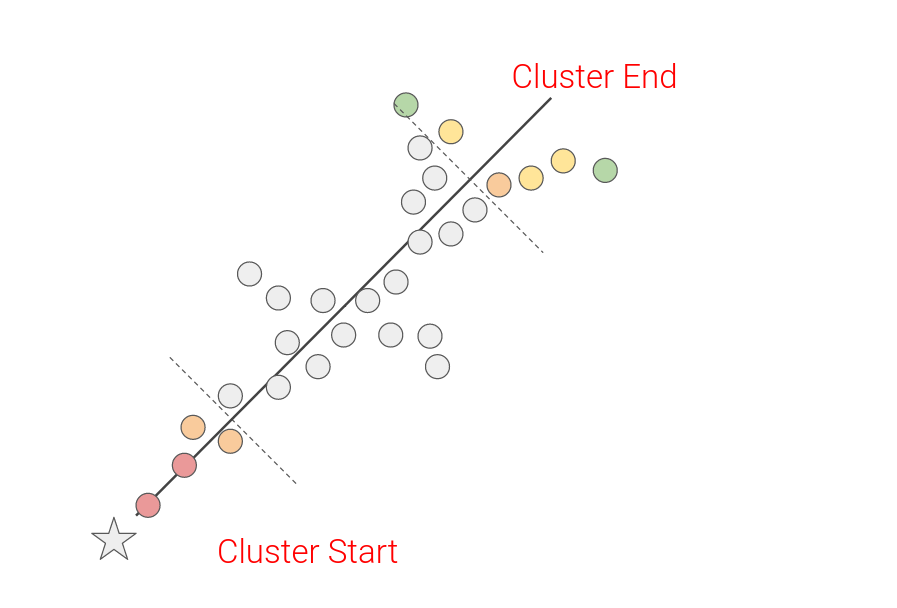
\includegraphics[width=\textwidth]{Conicalness}
            \caption{Conicalness}%
            \label{fig:conicalness}
        \end{subfigure}
        \caption[Cone-like Variable Diagrams]{
	Variables describing how cone-like the charge distribution is.
	}
        \label{fig:cone_variables}
\end{figure}


On top of the cone variables, another variable was added to the track-shower separation BDT to describe the hierarchy of the particle within a slice.
For a given particle, the daughters originating from that particle are identified and their number of hits are counted.
Distributions of the four new variables are shown in Fig. \ref{fig:bdt_features}, with track-like particles shown in blue and shower-like particles shown in red.
The concentration and conicalness variables display the strongest separation power between tracks and showers compared to the halo-total ratio and the number of daughter hits variables.

\begin{figure}[hb!]
        \centering
        \begin{subfigure}[b]{0.45\textwidth}
            \centering
            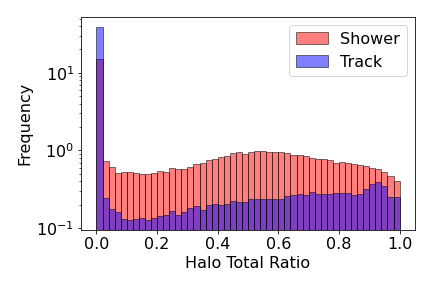
\includegraphics[width=\textwidth]{Feature_Halo_Total_Ratio}
            \caption{}%
        \end{subfigure}
        \hfill
        \begin{subfigure}[b]{0.45\textwidth}  
            \centering 
            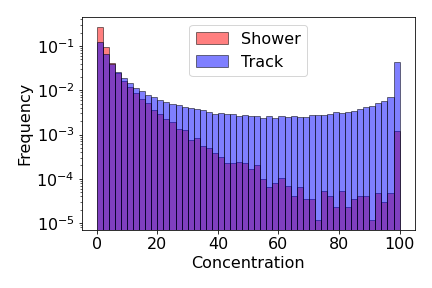
\includegraphics[width=\textwidth]{Feature_Concentration}
            \caption{}%
        \end{subfigure}
        \hfill
        \begin{subfigure}[b]{0.45\textwidth}  
            \centering 
            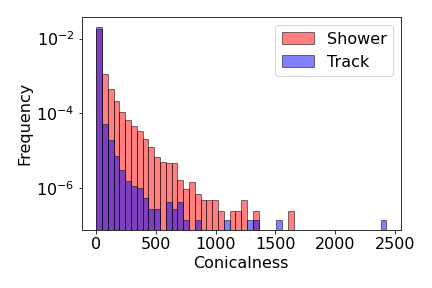
\includegraphics[width=\textwidth]{Feature_Conicalness}
            \caption{}%
        \end{subfigure}
        \hfill
        \begin{subfigure}[b]{0.45\textwidth}  
            \centering 
            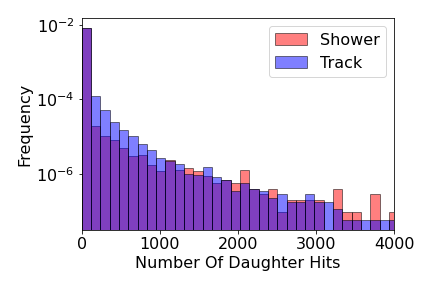
\includegraphics[width=\textwidth]{Feature_Number_Of_Daughter_Hits}
            \caption{}%
        \end{subfigure}
        \caption[New Variable Distributions of the Track-Shower Separation BDT]{
	Distributions of four new variables: (a) halo-total ratio, (b) concentration, (c) conicalness and (d) number of daughter hits.
	}
        \label{fig:bdt_features}
\end{figure}

Fig. \ref{fig:bdt_score} shows the score distribution of the BDT retrained with the four new variables.
The left figure shows two distinct distributions in red and blue for showers and tracks respectively.
This demonstrates a good separation power of the BDT, where particles with a score < 0.5 closely resemble showers whilst particles with a score > 0.5 are more track-like.
The score distribution is broken down into different particle types as shown in the right figure.
The distribution is expected given that electrons and photons leave electromagnetic shower activities inside the detector whilst charged particles like muons, charged pions and protons leave track-like signatures (See Section \ref{sec3:bethebloch}). 
The updated BDT resulted in a $0.1\sim2.0\%$ improvement in correctly classifying a particle type as shower-like or track-like.
The track-shower separation score distribution is used in downstream high level analysis tools as detailed in Section \ref{sec:subsystem_match} next.
It is also employed as a cut variable in the selection of Heavy Neutral Leptons (HNLs), to be discussed in Chapter \ref{ChapterSelect}.

\begin{figure}[htbp!]
        \centering
        \begin{subfigure}[b]{0.495\textwidth}
            \centering
            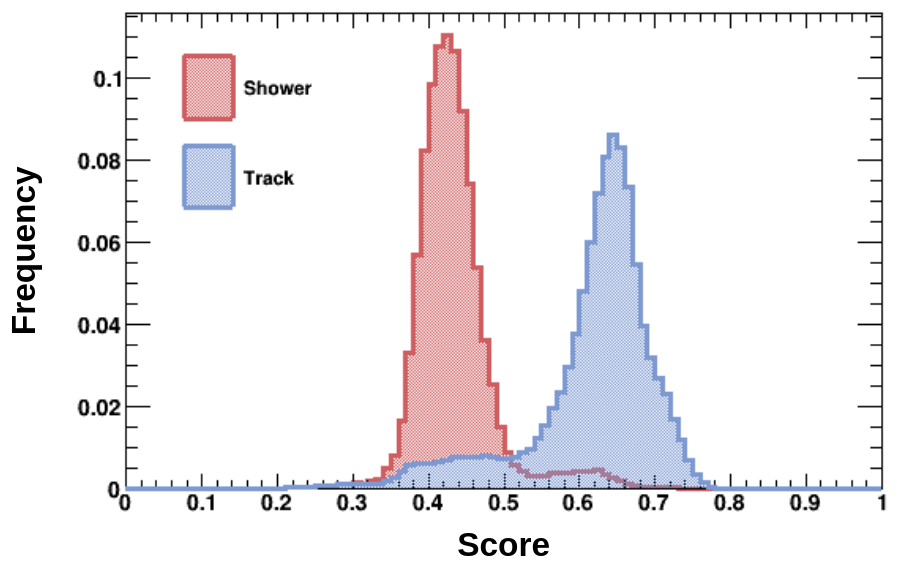
\includegraphics[width=\textwidth]{bdt_score_trk_shw}
            \caption{}%
        \end{subfigure}
        \hfill
        \begin{subfigure}[b]{0.495\textwidth}  
            \centering 
            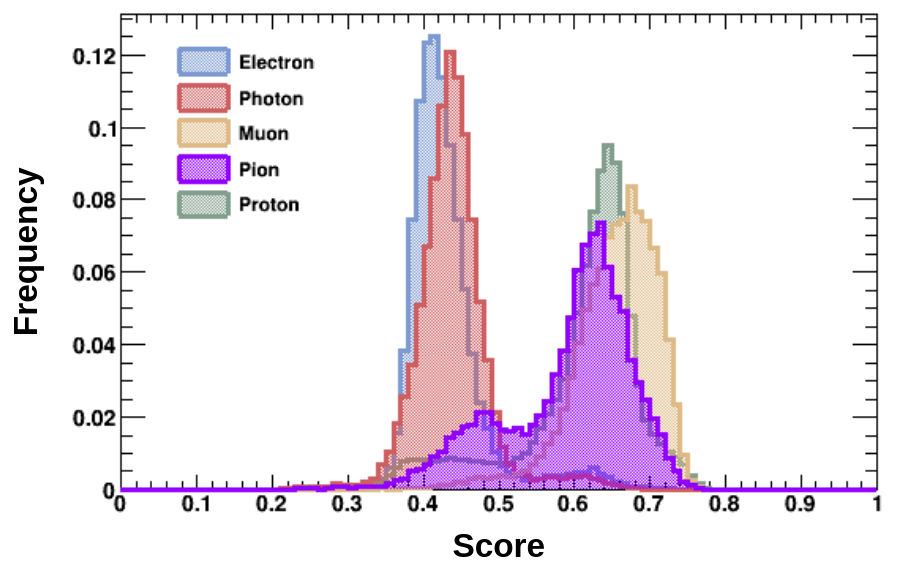
\includegraphics[width=\textwidth]{bdt_score_particle}
            \caption{}%
        \end{subfigure}
        \caption[Score Distributions of the Updated Track-Shower Separation BDT]{
	Score distribution of the updated track-shower BDT, plotted for (a) track-like and shower-like particles and (b) different particle types.
	}
        \label{fig:bdt_score}
\end{figure}

\section{Photon Detection System and Cosmic Ray Tagger Reconstruction}
\label{sec:reco_others}

The reconstruction workflows of the two detection subsystems, PDS and CRT, are given in Sections \ref{sec:reco_pds} and \ref{sec:crt_reco}. 

\subsection{Photon Detection System Reconstruction}
\label{sec:reco_pds}

%The reconstruction of optical detectors, PMTs and X-ARAPUCAs, shares the same steps of waveform deconvolution, hit finding and light reconstruction.
%However, different algorithms and parameter settings are required for each optical detector type due to their different responses.
Details on the PDS reconstruction at SBND can be found in Ref. \cite{sbnd_pds_paper}.
Here the focus is on the reconstruction of PMT waveforms, which have an averaged Single Electron Response (SER) pulse peaking at $\sim 25$ ADC and a full width at half maximum of $\sim$ 10 ns.
The fast response of PMT signals plays a key role in the nanosecond timing resolution requirement for the HNL search.

Fig. \ref{fig:pds_reco_deconvolution} depicts an example of a simulated PMT waveform before and after the deconvolution.% and baseline determination.
The top panel shows the number of \textit{true} PhotoElectrons (PEs) seen by a PMT as a function of time in green.
The middle panel figure shows the raw waveform in blue, convolved with the PMT response and noise.
%The AC circuits of PMTs lead to over/undershoot features across the raw waveform with respect to the baseline (See Section \ref{sec:pds_response}).
A 1D deconvolution and a high frequency filter are applied subsequently for noise removal.
The deconvolved waveform is shown in orange in the bottom panel, demonstrating that over/undershoot features are removed while peaks' magnitudes and positions are maintained.

Baseline of deconvolved PMT waveforms is estimated using the 400 ns portion at the start and end of the waveform.
Optical hits are identified after baseline subtraction, by finding pulses above the threshold of $1/4$ the amplitude of the deconvolved SER and 3 times the standard deviation of the baseline root mean square.
Fig. \ref{fig:pds_reco_hit_finding} depicts a simulated deconvolved and baseline-subtracted PMT waveform with five identified optical hits.
Peak times, corresponding to the maximum of an optical hit, are denoted with red triangles.
The first optical hit contains multiple peaks merged into a single optical hit due to multiple photons arriving very closely in time to the PMT.
The rise time of an optical hit is when its first peak goes above 15\% of its amplitude, denoted with blue stars.
It is an estimation of the arrival time of the first photon contributing to the optical hit. 
The integral of the optical hit is used to compute the number of PEs.
%which is calculated using a 400 ns portion at the start and end of the deconvolved waveform, resulting in the waveform shown in orange.
%This results in a resolution of 1.6 ns in estimating the arrival time of the first photon contributing to the optical hit.

\begin{figure}[hb!]
        \centering
        \begin{subfigure}[b]{0.59\textwidth}
            \centering
            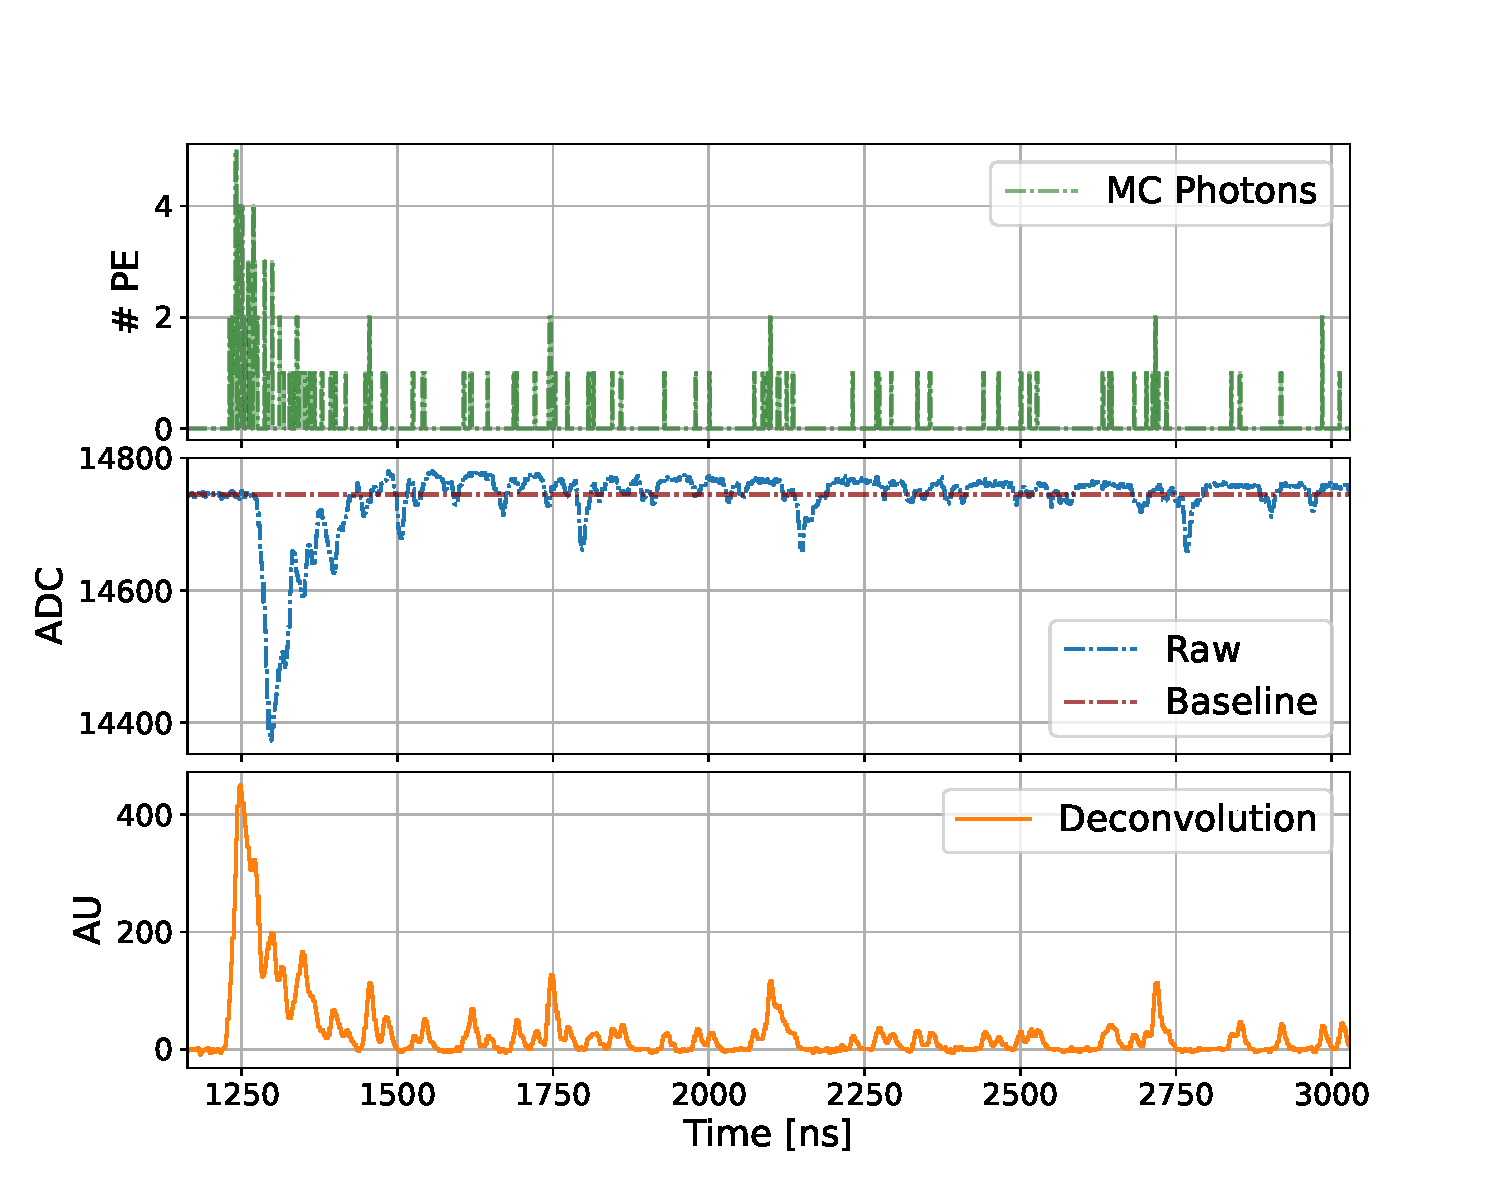
\includegraphics[width=\textwidth]{pds_reco_deconvolution}
            \caption{Waveform Deconvolution}
            \label{fig:pds_reco_deconvolution}
        \end{subfigure}
        \hfill
        \begin{subfigure}[b]{0.4\textwidth}  
            \centering 
            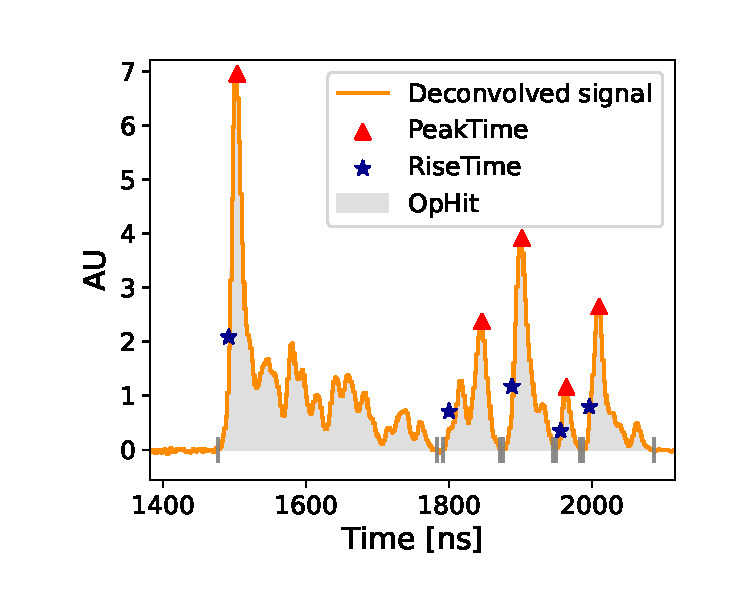
\includegraphics[width=\textwidth]{pds_reco_hit_finding}
            \caption{Hit Finding}
            \label{fig:pds_reco_hit_finding}
        \end{subfigure}
        \caption[Waveform Deconvolution and Hit Finding on PMT Waveforms]{
	Example demonstrating (a) waveform deconvolution and (b) hit finding applied to a PMT waveform \cite{sbnd_pds_paper}.
	}
        \label{fig:pds_reco}
\end{figure}


Optical hits from at least 3 PMTs are clustered into an \textit{optical flash}.
The length of an optical flash is set as 8 $\mu$s to account for the total light produced in a neutrino interaction in the TPC, from both prompt and slow components of scintillation photons.
The clustering algorithm is based on the number of PEs of optical hits, the timing distribution between hits and the geometrical location of the PMTs.
The number of PEs in a flash is the total PEs of hits clustered in that flash. 

The start time of the optical flash represents the start time of an interaction, $t_0$, which is the key variable of the HNL search, and therefore requires great care in reconstruction.
The flash start time is the average of the rise time of optical hits in a flash, only considering PMTs that contribute 50\% of the prompt light in the 30 ns window of the largest number of PEs.
A correction is applied for the propagation of the photons from the scintillation location to the PMTs.

The correction is computed by exploiting the high density of PMTs as well as having coated and uncoated PMTs sensitive to direct VUV light and reflected visible light (See Section \ref{sec:sbnd_pds}).
Fig. \ref{fig:light_yield_Diego} shows the reconstructed light yield seen by coated and uncoated PMTs based on simulation, as a function of the photon mean drift distance, $d_{drift}$.
The error bars show the uncertainty due to the geometrical effects of the detector.

Closer to the anode at $d_{drift} = 0 $ cm, the light yield primarily comes from direct VUV photons, detected by coated PMTs as shown in purple.
Closer to the cathode at $d_{drift} = 200 $ cm, and hence to the reflective foils, the light yield from reflected visible photons increases, detected by uncoated PMTs as shown in red.
For a given scintillation location, the amount of direct VUV and visible photons leads to a specific ratio of the two components, which is used to compute the correction for the drift propagation effect.
The resulting timing resolution of the flash time is $\mathcal{O}$(2 ns) across the drift distance, demonstrating the excellent capability of the PDS reconstruction at SBND \cite{sbnd_pds_paper}.

\begin{figure}[hb!]
\centering    
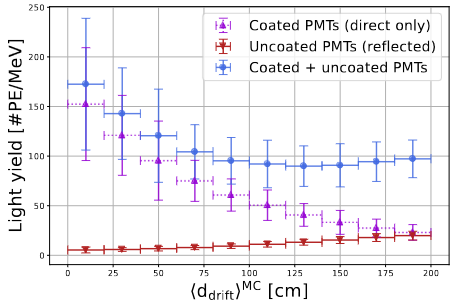
\includegraphics[width=0.55\textwidth]{light_yield_sim}
\caption[Reconstructed Light Yield at SBND]{
Reconstructed light yield as a function of the mean drift distance based on simulation \cite{sbnd_pds_paper}. 
}
\label{fig:light_yield_Diego}
\end{figure}


\subsection{Cosmic Ray Tagger Reconstruction}
\label{sec:crt_reco}

The CRT reconstruction is the simplest of the three detection subsystems.
Outputs of the CRT readout electronics are in a group of 32 ADC values, for a single ADC per SiPM (See Section \ref{sec:readout}).
The reconstruction begins with a hit finding algorithm to identify which pair of SiPMs in the group goes above a threshold.
The SiPM pair determines the lateral position of a cosmic muon hit within a CRT strip.
A clustering algorithm groups hits from orthogonal CRT strips of the same wall within a 50 ns window to yield 3D space points.
For each CRT space point, the timing and calorimetry information is calculated and corrected for the propagation effect from the hit position to the SiPM.
CRT space points from multiple CRT walls are matched together to form a CRT track based on the timing agreement and prioritising three-point tracks over two-point tracks.
The outputs are both CRT space points and tracks. 

%The final step is to match space points from multiple CRT walls to form a CRT track.
%Candidate tracks are evaluated from any combinations of space points from different walls within a 100 ns coincidence window.
%The best track candidate is selected by the goodness of timing agreement and prioritising three-point tracks over two-point tracks. 

%********************************** %First Section  **************************************
\section{High Level Analysis Tools}
\label{sec:reco_ana_tools}

Reconstructed variables from each detection subsystem: slices from the TPC, flashes from the PDS, space points and tracks from the CRTs, are used collectively by downstream algorithms to compute useful characteristics regarding the interaction.
This section covers the main high level analysis tools used in the selection of HNLs, to be detailed in Chapter \ref{ChapterSelect}.
Section \ref{sec:subsystem_match} provides a description of on how variables from different detection subsystems can be matched to the same interaction.
Presented in Section \ref{sec:crumbs} is the cosmic rejection tool.
Particle identification tool is given Section \ref{sec:razzled} .

\subsection{Subsystem Matching}
\label{sec:subsystem_match}

%Another example is that tracks produced in the TPC deposit energy in the nearest CRT strips only when they enter or exit the detector, enabling the tagging of stopping or exiting particles.

Reconstructed tracks from the TPC reconstruction can be matched to a CRT space point or tracks to provide additional information for cosmic rejection.
An example is that a through-going cosmic muon produces a long track in the TPC as well as deposits energy in the nearest CRT walls where the track starts and ends. 
Two types of TPC-CRT matching are performed: (1) matching a TPC track to CRT space points and (2) matching a TPC track to CRT tracks.
The former method extrapolates the TPC track and matches with the nearest CRT space points by computing a Distance of Closest Approach (DCA), confining the matching to a single CRT wall. 
The latter method uses a compound score from the DCA of a TPC track to many CRT tracks and the angle between them, enabling matching a TPC track to many CRT walls.
Both methods use the CRT timing information for further constraints and no matching duplications are allowed.

An interaction reconstructed using the TPC, a slice, can be matched to an interaction reconstructed using PMTs, an optical flash, referred to as \textit{slice-to-flash} matching.
The flash time matched to a slice represents the start time of the interaction reconstructed in that slice.
It is the key variable to compute the arrival time of a particle, enabling the reconstruction of the bucket structure of the Booster Neutrino Beam.

%to light yield based on the topology of particles in the slice.
%The track score of the particles in the slice, assigned by the track-shower separation BDT (See Section \ref{sec:trkshwbdt}), determines which calorimetry computation is appropriate (See Section \ref{sec:pandora}).
%If the particle is track-like, the calorimetry computation uses the modified Box recombination formalism with the charge-light anti-correlation. 
%If the particle is shower-like, the calorimetry computation uses a charge-to-light conversion by multiplying a constant.     
The slice-to-flash matching is based on the prediction of number of PEs estimated from the measured charge in a slice, and whether it is in good agreement with the number of PEs measured by PMTs \cite{opt0finder_module}.
The measured charge of a slice is first converted to deposited energy, which is then used compute the total light produced from an interaction.
The semi-analytical light library is re-run to estimate the number of PEs that would be measured by PMTs.
This results in the number of PEs predicted from the measured charged, referred to as $L_{\mathrm{Q}}$.
The prediction is compared to the number of PEs measured by PMTs $L$ of any given flash by a $\chi^2$ computation.
The flash best matched to a slice has the lowest $\chi^2$.
Only one-to-one match is allowed so that only a single flash is matched to a slice.

A useful fraction variable is computed from $L_{\mathrm{Q}}$ and $L$ as follows:
\begin{equation}
\label{eq:opt0fraction}
        \frac{L_{\mathrm{Q}} - L}{L}.
\end{equation}
This fraction indicates the level of agreement between $L_{\mathrm{Q}}$ and $L$, and thus, the level of agreement of the energy deposition reconstructed from the measured charge and the measured light.
If the fraction is positive, the predicted light from the measured charge is overestimated compared to the measured light, otherwise, it is underestimated.
This variable is particularly useful in the selection of HNL signals as it enables the identification of boosted topologies.

\subsection{Cosmic Rejection}
\label{sec:crumbs}

Cosmic Rejection Using a Multi-system Boosted decision tree Score (CRUMBS) is a binary classification BDT that outputs a score whether a reconstructed slice is cosmic-like or neutrino-like \cite{crumbs}. 
Reconstruction variables from all three detection subsystems that are complementary to each other are input into CRUMBS, thereby reducing inefficiencies compared to using a single subsystem.
The TPC information includes variables describing a particle as both neutrino-like and cosmic-like, accounting for its charge distribution, location within the TPC and deposited energy.  
The PDS information is from the flash best matched to the slice of interest, particularly the number of PEs in the flash and the $\chi^{2}$ from the slice-to-flash matching.                        
The CRT information consists of both TPC-CRT matching algorithms, including the timing information of the CRT space points/tracks and the matching score.
The score distribution of CRUMBS shows a significant separation between neutrino-like signals and cosmic-like backgrounds, enabling an effective cosmic rejection (See Fig. \ref{fig:crumbs_cut}, Section \ref{sec:cosmic_crumbs}).

%CRUMBS was trained using the TMVA toolkit \cite{tmva} on MC samples of neutrinos, evenly distributed between $CC\nu_{\mu}$ and $CC\nu_{e}$, and cosmic muons.

\subsection{Particle Identification}
\label{sec:razzled}

The main particle identification tool at SBND is called Razzled \cite{razzled}, which is a multi-classification BDT designed to identify five particle types: $e$, $\gamma$, $\mu$, $\pi$ and $p$.
The reconstruction variables input into Razzled are only TPC reconstruction variables from the Pandora package.
There are three categories of variables for training Razzled: (1) generic reconstruction variables, (2) track-like variables and (3) shower-like variables.
The generic variables describe the particle multiplicity, topology, directionality and charge distribution.
Track variables include track lengths, energy deposition, kinematics in the stopping region to identify Bragg peak, and multiple Coulomb scattering for $\mu$-$\pi$ separation.
Shower variables include shower conversion gaps, opening angles and energy deposition aiming towards $\gamma$-$e$ separation.
This collection of variables allows Razzled to exploit the correlation between variables, thereby significantly improving the identification performance over traditional hand cuts.
A full description of the input variables and its performance can be found in Ref. \cite{EdPhD}.
For each reconstructed particle, Razzled outputs a score for each particle type and assigns the highest particle type score to that particle.

\section{Concluding Remarks}
\label{sec:reco_concluding_remarks}

The reconstruction workflow of SBND is described, outlining the reconstruction process for each detection system: the TPC, PDS and CRTs.
The three detection subsystems together provide complementary information regarding the underlying reconstructed interaction and are used collectively by different analysis tools for various purposes.
Focusing on the selection of HNLs, the background rejection and signal selection employ the tools described here to achieve a high signal-to-background ratio as discussed later in Chapter \ref{ChapterSelect}.

Particularly, the most important variable is the reconstructed interaction time, $t_0$, which is used to compute the arrival time at the front face of SBND.
The timing reconstruction having a resolution $\mathcal{O}$(2 ns) is able to resolve the Gaussian-shaped bucket of SM neutrinos.
To achieve such high timing resolution at the high level reconstruction, the low level readout electronics must have sufficient timing resolution to maintain a high quality data stream at a high sampling rate.
The timing performance of the readout electronics is discussed in Chapter \ref{ChapterDAQ} next.

%The event building process of the DAQ relies on the timing information acquired from each subsystem. 
%This process assembles the foundation of physics event upon which low level and high level reconstructions are built to achieve nanosecond timing resolution.
